\documentclass{beamer}
% =============================================================================
% ENCODING
% =============================================================================
\usepackage[utf8]{inputenc}  % UTF-8 encoding support

% =============================================================================
% GRAPHICS
% =============================================================================
\usepackage{graphicx}  % For \includegraphics (401 uses across lectures)

% =============================================================================
% MATH PACKAGES
% =============================================================================
\usepackage{amsmath}    % For align, multline, equation environments (heavily used)
\usepackage{amsfonts}   % For \mathbb (e.g., \bbR, \bbE)
\usepackage{amssymb}    % For additional math symbols

% =============================================================================
% TABLES
% =============================================================================
\usepackage{booktabs}   % For \toprule, \midrule, \bottomrule (used in lecture13, lecture14)

% =============================================================================
% LISTS
% =============================================================================
\usepackage{enumerate}  % Enhanced enumerate environment (76 uses across lectures)

% =============================================================================
% TIKZ (DIAGRAMS)
% =============================================================================
\usepackage{tikz}       % For taxonomy diagram and footnotes positioning

% =============================================================================
% UTILITY PACKAGES
% =============================================================================
\usepackage{multido}    % For \multido command used in \eqpause
\usepackage{etoolbox}   % For \AtEndEnvironment, \ifbool, \newbool (used in preamble and taxonomy)

% =============================================================================
% BEAMER THEME SETTINGS
% =============================================================================
\usetheme{default}
\usecolortheme{default}

\setbeamerfont{title}{size=\Huge}
\setbeamertemplate{footline}[frame number]{}
\setbeamertemplate{section in toc}[sections numbered]

\makeatletter
\newcommand\HUGE{\@setfontsize\Huge{35}{40}}
\makeatother    

\setbeamerfont{title}{size=\HUGE}
\beamertemplatenavigationsymbolsempty

% =============================================================================
% TIKZ LIBRARIES
% =============================================================================
% Used for taxonomy diagram: arrows, positioning, shapes
\usetikzlibrary{arrows.meta,calc,shapes,positioning,shadows,trees}

% =============================================================================
% CUSTOM FOOTNOTE COMMANDS
% =============================================================================
% \myfootnote{text} - creates a footnote at the bottom of the slide
\newcommand\myfootnote[1]{%
  \vspace{-0.5cm}%
  \tikz[remember picture,overlay]
  \draw (current page.south west) +(1in + \oddsidemargin,0.5em)
  node[anchor=south west,inner sep=0pt]{\parbox{\textwidth}{%
      \rlap{\rule{10em}{0.4pt}}\raggedright\scriptsize \textit{#1}}};}

% \myfootnotewithlink{url}{text} - creates a clickable footnote (623 uses across lectures)
\newcommand\myfootnotewithlink[2]{%
  \vspace{-0.5cm}%
  \tikz[remember picture,overlay]
  \draw (current page.south west) +(1in + \oddsidemargin,0.5em)
  node[anchor=south west,inner sep=0pt]{\parbox{\textwidth}{%
      \rlap{\rule{10em}{0.4pt}}\raggedright\scriptsize\href{#1}{\textit{#2}}}};}

% =============================================================================
% SECTION/SUBSECTION OUTLINE AUTOMATION
% =============================================================================
% Automatically show outline at the beginning of each section
\AtBeginSection[]
      {
      	\begin{frame}{Outline}
      		\tableofcontents[currentsection]
      	\end{frame}
      }
      \AtBeginSubsection[]{
      	\begin{frame}{Outline}
      		\tableofcontents[currentsection,currentsubsection]
      	\end{frame}
}

% =============================================================================
% CUSTOM SLIDE ANIMATION COMMANDS
% =============================================================================
% These commands enable step-by-step reveal of equations and content
% Used heavily across all lectures (1130+ uses of \nextonslide and \eqpause)

\newcounter{noscounter}   % Counter for \nextonslide (resets on each new slide)
\newcounter{pcounter}     % Counter for pause commands (resets after \eqpause)
\newcounter{diffcounter}  % Counts pauses after equations

% \nextonslide{content} - reveals content on the next overlay
\newcommand{\nextonslide}[1]{%
  \stepcounter{noscounter}%
  \stepcounter{pcounter}%
  \stepcounter{diffcounter}%
  \onslide<\value{noscounter}->{#1}%
}

% \resetonslide - resets all animation counters (called at each frame)
\newcommand{\resetonslide}{%
    \setcounter{noscounter}{1}%
    \setcounter{pcounter}{1}%
    \setcounter{diffcounter}{0}%
}

% \eqpause - pause after equation that syncs with \nextonslide
\newcommand{\eqpause}{%
  \multido{\i=1+1}{\value{pcounter}}{\pause}%
  \stepcounter{noscounter}%
  \setcounter{pcounter}{1}%
}

% \eqpausediff - helper command, runs automatically after math environments
\newcommand{\eqpausediff}{%
  \multido{\i=1+1}{\value{diffcounter}}{\pause}%
  \addtocounter{pcounter}{-\value{diffcounter}}%
  \setcounter{diffcounter}{0}%
}

% Apply \eqpausediff after math environments
\newcommand\AtEndBoth[2]{%
  \AtEndEnvironment{#1}{#2}%
  \AtEndEnvironment{#1*}{#2}%
}

\AtEndBoth{align}{\eqpausediff}
\AtEndBoth{equation}{\eqpausediff}
\AtEndBoth{multline}{\eqpausediff}

% Reset counters at the beginning of each frame
\addtobeamertemplate{frametitle}{\resetonslide}{}

% =============================================================================
% INCLUDE OTHER CONFIGURATION FILES
% =============================================================================
% ==============================================================================
% Custom LaTeX Commands for Deep Generative Models Course
% ==============================================================================

% ==============================================================================
% BOLD LETTERS (mathbf / boldsymbol)
% ==============================================================================

% ------------------------------------------------------------------------------
% Latin Bold Lowercase
% Usage: \bx for x in bold, commonly used for vectors
% ------------------------------------------------------------------------------
\newcommand{\ba}{\mathbf{a}}
\newcommand{\bc}{\mathbf{c}}
\newcommand{\be}{\mathbf{e}}
\newcommand{\bff}{\mathbf{f}}  % Note: \bf is reserved for bold font switching
\newcommand{\bg}{\mathbf{g}}
\newcommand{\bh}{\mathbf{h}}
\newcommand{\bp}{\mathbf{p}}
\newcommand{\bq}{\mathbf{q}}
\newcommand{\bs}{\mathbf{s}}
\newcommand{\bt}{\mathbf{t}}
\newcommand{\bu}{\mathbf{u}}
\newcommand{\bv}{\mathbf{v}}
\newcommand{\bw}{\mathbf{w}}
\newcommand{\bx}{\mathbf{x}}
\newcommand{\by}{\mathbf{y}}
\newcommand{\bz}{\mathbf{z}}

% ------------------------------------------------------------------------------
% Latin Bold Uppercase
% Usage: \bX for X in bold, commonly used for matrices or random vectors
% ------------------------------------------------------------------------------
\newcommand{\bA}{\mathbf{A}}
\newcommand{\bG}{\mathbf{G}}
\newcommand{\bI}{\mathbf{I}}
\newcommand{\bJ}{\mathbf{J}}
\newcommand{\bL}{\mathbf{L}}
\newcommand{\bM}{\mathbf{M}}
\newcommand{\bP}{\mathbf{P}}
\newcommand{\bQ}{\mathbf{Q}}
\newcommand{\bR}{\mathbf{R}}
\newcommand{\bT}{\mathbf{T}}
\newcommand{\bU}{\mathbf{U}}
\newcommand{\bV}{\mathbf{V}}
\newcommand{\bW}{\mathbf{W}}
\newcommand{\bX}{\mathbf{X}}
\newcommand{\bZ}{\mathbf{Z}}

% ------------------------------------------------------------------------------
% Greek Bold Lowercase
% Usage: \btheta for θ in bold, commonly used for parameter vectors
% ------------------------------------------------------------------------------
\newcommand{\bepsilon}{\boldsymbol{\epsilon}}
\newcommand{\blambda}{\boldsymbol{\lambda}}
\newcommand{\bmu}{\boldsymbol{\mu}}
\newcommand{\bphi}{\boldsymbol{\phi}}
\newcommand{\bpi}{\boldsymbol{\pi}}
\newcommand{\bpsi}{\boldsymbol{\psi}}
\newcommand{\bsigma}{\boldsymbol{\sigma}}
\newcommand{\btheta}{\boldsymbol{\theta}}

% ------------------------------------------------------------------------------
% Greek Bold Uppercase
% Usage: \bSigma for Σ in bold, commonly used for covariance matrices
% ------------------------------------------------------------------------------
\newcommand{\bSigma}{\boldsymbol{\Sigma}}
\newcommand{\bTheta}{\boldsymbol{\Theta}}

% ==============================================================================
% CALLIGRAPHIC LETTERS (mathcal)
% Usage: \cX for calligraphic X, commonly used for sets and spaces
% ==============================================================================
\newcommand{\cF}{\mathcal{F}}
\newcommand{\cI}{\mathcal{I}}
\newcommand{\cL}{\mathcal{L}}
\newcommand{\cM}{\mathcal{M}}
\newcommand{\cN}{\mathcal{N}}
\newcommand{\cP}{\mathcal{P}}
\newcommand{\cS}{\mathcal{S}}
\newcommand{\cT}{\mathcal{T}}
\newcommand{\cW}{\mathcal{W}}
\newcommand{\cX}{\mathcal{X}}
\newcommand{\cZ}{\mathcal{Z}}

% ==============================================================================
% BLACKBOARD BOLD LETTERS (mathbb)
% Usage: \bbR for ℝ, commonly used for number sets and expectations
% ==============================================================================
\newcommand{\bbE}{\mathbb{E}}  % Expectation
\newcommand{\bbI}{\mathbb{I}}  % Indicator function
\newcommand{\bbP}{\mathbb{P}}  % Probability measure
\newcommand{\bbR}{\mathbb{R}}  % Real numbers

% ==============================================================================
% MATH OPERATORS
% ==============================================================================

% ------------------------------------------------------------------------------
% Optimization Operators
% Usage: \argmin_{x} f(x) for proper spacing and limits placement
% ------------------------------------------------------------------------------
\DeclareMathOperator*{\argmin}{arg\,min}
\DeclareMathOperator*{\argmax}{arg\,max}

% ------------------------------------------------------------------------------
% Statistical Operators
% Usage: \cov(X, Y) for covariance
% ------------------------------------------------------------------------------
\DeclareMathOperator{\cov}{cov}

% ------------------------------------------------------------------------------
% Linear Algebra Operators
% Usage: \tr(\bA) for trace of matrix A
% ------------------------------------------------------------------------------
\DeclareMathOperator{\tr}{tr}

% ------------------------------------------------------------------------------
% Other Mathematical Operators
% ------------------------------------------------------------------------------
\DeclareMathOperator{\diver}{div}      % Divergence (vector calculus)
\DeclareMathOperator{\softmax}{softmax}
\DeclareMathOperator{\supp}{supp}      % Support of a distribution

% ==============================================================================
% PROBABILITY DISTRIBUTIONS
% Usage: X \sim \cN(0, 1), Y \sim \Bern(p)
% ==============================================================================
\DeclareMathOperator{\Bern}{Bern}      % Bernoulli distribution
\DeclareMathOperator{\Cat}{Cat}        % Categorical distribution
\DeclareMathOperator{\Gumbel}{Gumbel}  % Gumbel distribution
\DeclareMathOperator{\Uniform}{Uniform}

% ==============================================================================
% METRICS AND DIVERGENCES
% Usage: \KL(p \| q), \JSD(p, q)
% ==============================================================================
\newcommand{\Ent}{\mathrm{H}}          % Entropy
\newcommand{\FID}{\mathrm{FID}}        % Fréchet Inception Distance
\newcommand{\JSD}{\mathrm{JSD}}        % Jensen-Shannon Divergence
\newcommand{\KL}{\mathrm{KL}}          % Kullback-Leibler Divergence
\DeclareMathOperator{\MMD}{MMD}        % Maximum Mean Discrepancy
\DeclareMathOperator{\SNR}{SNR}        % Signal-to-Noise Ratio

% ==============================================================================
% NEURAL NETWORK NOTATION
% ==============================================================================

% ------------------------------------------------------------------------------
% Network Architectures (upright font for abbreviations)
% Usage: f_{\btheta} = \NN_{\btheta}(\bx)
% ------------------------------------------------------------------------------
\newcommand{\MLP}{\mathrm{MLP}}        % Multi-Layer Perceptron
\newcommand{\NN}{\mathrm{NN}}          % Neural Network
\newcommand{\RNN}{\mathrm{RNN}}        % Recurrent Neural Network

% ------------------------------------------------------------------------------
% Numerical Solvers (monospace font)
% Usage: \bx_T = \ODESolve(f, \bx_0, T)
% ------------------------------------------------------------------------------
\newcommand{\ODESolve}{\texttt{ODESolve}}
\newcommand{\SDESolve}{\texttt{SDESolve}}

% ==============================================================================
% COMMON SHORTCUTS
% Usage: Frequently used subscripted or parameterized expressions
% ==============================================================================
\newcommand{\pd}{p_{\text{data}}}              % Data distribution
\newcommand{\pt}{p_{\boldsymbol{\theta}}}      % Parameterized distribution
\newcommand{\qagg}{q_{\text{agg}}}             % Aggregated posterior
\newcommand{\lambdamax}{\lambda_{\text{max}}}  % Maximum eigenvalue
  % Math shorthand commands (\bx, \bbE, \KL, etc.)
\input{../utils/title}        % Title page template
\centering
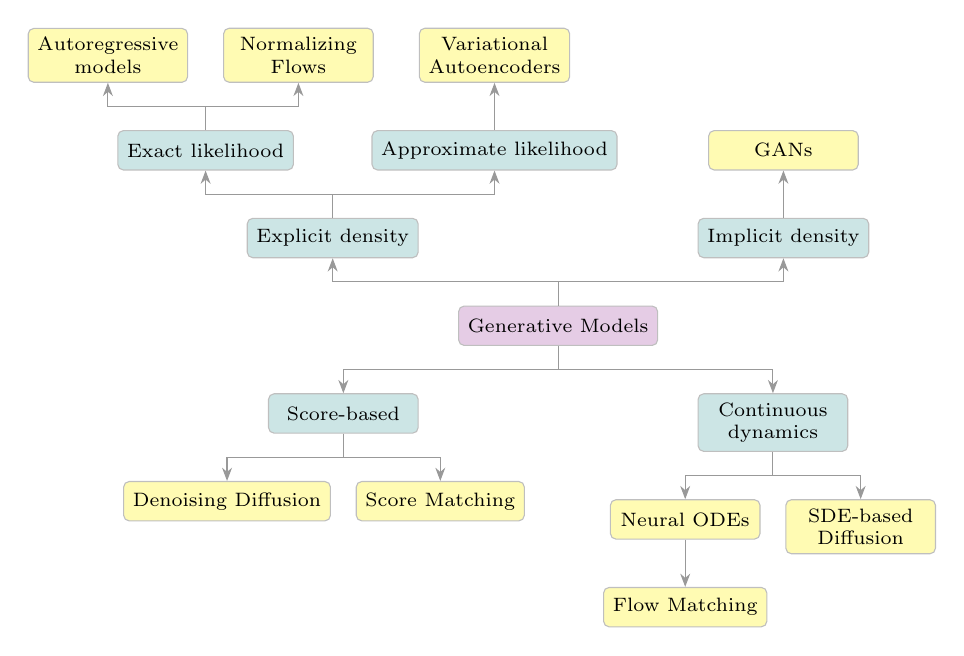
\begin{tikzpicture}[
    scale=1.0, transform shape,
    node distance=0.6cm and 0.3cm,
    box/.style={
        rectangle, 
        draw=gray!50, 
        rounded corners=2pt, 
        minimum width=1.9cm, 
        minimum height=0.5cm, 
        align=center, 
        font=\scriptsize, 
        line width=0.4pt
    },
    root/.style={box, fill=violet!20},
    category/.style={box, fill=teal!20},
    model/.style={box, fill=yellow!30},
    arrow/.style={-Stealth, draw=gray!80, line width=0.4pt}
]

    % --- CENTRAL ROOT ---
    \node[root] (root) {Generative Models};

    % --- UPPER BRANCHES (SWAPPED) ---
    % Tier 1: Explicit (Left) and Implicit (Right)
    \node[category, above left=0.6cm and 0.5cm of root] (explicit) {Explicit density};
    \node[category, above right=0.6cm and 0.5cm of root] (implicit) {Implicit density};

    % Tier 2 (Left side: Likelihoods)
    \node[category, above left=0.6cm and -0.6cm of explicit] (exact) {Exact likelihood};
    \node[category, above right=0.6cm and -0.6cm of explicit] (approx) {Approximate likelihood};

    % Tier 2 (Right side: GANs)
    \node[model, above=0.6cm of implicit] (gans) {GANs};

    % Tier 3 (Final Models Up)
    \node[model, above left=0.6cm and -0.9cm of exact] (ar) {Autoregressive \\ models};
    \node[model, above right=0.6cm and -0.9cm of exact] (nf) {Normalizing \\ Flows};
    \node[model, above=0.6cm of approx] (vae) {Variational \\ Autoencoders};

    % --- LOWER BRANCHES ---
    % Tier 1: Score-based and Continuous
    \node[category, below left=0.6cm and 0.5cm of root] (score) {Score-based};
    \node[category, below right=0.6cm and 0.5cm of root] (cont) {Continuous \\ dynamics};

    % Tier 2 (Score Models)
    \node[model, below left=0.6cm and -0.8cm of score] (ddpm) {Denoising Diffusion};
    \node[model, below right=0.6cm and -0.8cm of score] (sm) {Score Matching};

    % Tier 2 (Continuous Models)
    \node[model, below left=0.6cm and -0.8cm of cont] (node) {Neural ODEs};
    \node[model, below right=0.6cm and -0.8cm of cont] (sde) {SDE-based \\ Diffusion};

    % Tier 3 (Flow Matching)
    \node[model, below=0.6cm of node] (fm) {Flow Matching};

    % --- CONNECTIONS ---
    % Root to Tier 1
    \draw[arrow] (root.north) -- ++(0,0.3) -| (explicit.south);
    \draw[arrow] (root.north) -- ++(0,0.3) -| (implicit.south);
    \draw[arrow] (root.south) -- ++(0,-0.3) -| (score.north);
    \draw[arrow] (root.south) -- ++(0,-0.3) -| (cont.north);

    % Explicit side connections
    \draw[arrow] (explicit.north) -- ++(0,0.3) -| (exact.south);
    \draw[arrow] (explicit.north) -- ++(0,0.3) -| (approx.south);
    \draw[arrow] (exact.north) -- ++(0,0.3) -| (ar.south);
    \draw[arrow] (exact.north) -- ++(0,0.3) -| (nf.south);
    \draw[arrow] (approx.north) -- (vae.south);

    % Implicit side connection
    \draw[arrow] (implicit.north) -- (gans.south);

    % Score side connections
    \draw[arrow] (score.south) -- ++(0,-0.3) -| (ddpm.north);
    \draw[arrow] (score.south) -- ++(0,-0.3) -| (sm.north);

    % Continuous side connections
    \draw[arrow] (cont.south) -- ++(0,-0.3) -| (node.north);
    \draw[arrow] (cont.south) -- ++(0,-0.3) -| (sde.north);
    \draw[arrow] (node.south) -- (fm.north);

\end{tikzpicture}     % Generative models taxonomy diagram

\createdgmtitle{14}

\usepackage{tikz}
\usetikzlibrary{arrows.meta,positioning,fit}
%--------------------------------------------------------------------------------
\begin{document}
%--------------------------------------------------------------------------------
\begin{frame}[noframenumbering,plain]
\titlepage
	\resetonslide
\end{frame}
%=======
\begin{frame}{Recap of Previous Lecture}
	\myfootnotewithlink{https://arxiv.org/abs/2210.02747}{Lipman Y., et al. Flow Matching for Generative Modeling, 2022}
	\[
		\bbE_{\pd(\bx(0))} \bbE_{t \sim U[0, 1]} \bbE_{q(\bx(t) | \bx(0))}\bigl\| \bs_{\btheta}(\bx(t), t) - {\color{teal}\nabla_{\bx(t)} \log q(\bx(t) | \bx(0))} \bigr\|^2_2 
	\]
	\vspace{-0.3cm}
	\[
		p_t(\bx| \bx_1) = q_{1-t}(\bx| \bx_0=\bx_1)
	\]
	\vspace{-0.5cm}
	\begin{block}{Variance Exploding SDE}
		\vspace{-0.7cm}
		\[
				p_t(\bx | \bx_1) = \cN\left(\bx_1, \sigma^2_{1-t}  \bI\right) \quad \Rightarrow \quad 
				\bff(\bx, \bx_1, t) = - \frac{\sigma'_{1-t}}{\sigma_{1-t}} (\bx_t - \bx_1)
		\]
		\vspace{-0.7cm}
	\end{block}
	\begin{block}{Variance Preserving SDE}
		\vspace{-0.7cm}
		{\small
		\[
			p_t(\bx_t | \bx_1) = \cN\left(\alpha_{1-t}  \bx_1, (1 - \alpha^2_{1-t})  \bI \right)  \, \Rightarrow \, 
		\bff(\bx_t, \bx_1, t) = \frac{\alpha'_{1-t}}{1 - \alpha^2_{1-t}}\cdot \left(\alpha_{1-t}  \bx_t - \bx_1\right)
		\]
		}
	\end{block}
	\vspace{-0.5cm}
	\begin{figure}
		\centering
		\includegraphics[width=0.5\linewidth]{figs/trajectories}
	\end{figure}
\end{frame}
%=======
\begin{frame}{Recap of Previous Lecture}
	\begin{block}{Continuous state space}
		\begin{itemize}
			\item \textbf{Discrete time} $t \in \{0,1,\ldots,T\}$ $\;\Rightarrow\;$ \textbf{DDPM / NCSN}.
			\item \textbf{Continuous time} $t \in [0,1]$ $\;\Rightarrow\;$ \textbf{Score-based SDE models}.
		\end{itemize}
	\end{block}
	\begin{block}{Discrete state space}
		\begin{itemize}
			\item \textbf{Discrete time} $t \in \{0,1,\ldots,T\}$.
			\item \textbf{Continuous time} $t \in [0,1]$.
		\end{itemize}
	\end{block}
    \begin{block}{Key advantages of discrete diffusion}
		\begin{itemize}
			\item Parallel generation
			\item Flexible infilling
			\item Robustness
			\item Unified framework
        \end{itemize}
	\end{block}
\end{frame}
%=======
\begin{frame}{Recap of Previous Lecture}
	\myfootnotewithlink{https://arxiv.org/abs/2107.03006}{Austin J. et al. Structured denoising diffusion models in discrete state-spaces, 2021.}
	\begin{block}{Discrete Diffusion Markov Chain}
		\[
			q(\bx_t|\bx_{t-1}) = \Cat(\bQ_t\bx_{t-1}),
		\]
        Each $\bx_t \in \{0,1\}^K$ is a \textbf{one-hot vector} encoding the categorical state (it is just one token).
	\end{block}
    \begin{block}{Transition Matrix}
		\vspace{-0.5cm}
		\[
			[\bQ_t]_{ij} = q(x_t = i | x_{t-1} = j),
			\qquad
			\sum_{i=1}^K [\bQ_t]_{ij} = 1.
		\]
        \[
            q(\bx_t|\bx_0) = \Cat(\bQ_{1:t}\bx_0),
            \qquad
            \bQ_{1:t} = \bQ_t \bQ_{t-1}\cdots\bQ_1.
        \]
		\vspace{-0.5cm}
	\end{block}
    \begin{itemize}
		\item The choice of $\bQ_t$ determines how information is erased and what the stationary distribution becomes.
		\item $\bQ_t$ and $\bQ_{1:t}$ should be easy to compute for each $t$.
	\end{itemize}
\end{frame}
%=======
\begin{frame}{Recap of Previous Lecture}
	\myfootnotewithlink{https://arxiv.org/abs/2107.03006}{Austin J. et al., Structured denoising diffusion models in discrete state-spaces, 2021.}
	\begin{block}{Uniform vs. Absorbing Transition Matrix}
        \begin{table}[h!]
            \centering
            \small
            \begin{tabular}{lcc}
                \toprule
                \textbf{Aspect} & \textbf{Uniform Diffusion} & \textbf{Absorbing Diffusion} \\
                \midrule
                $\bQ_t$
                    & $(1-\beta_t)\bI + \beta_t \mathbf{U}$ 
                    & $(1-\beta_t)\bI + \beta_t \mathbf{e}_m\mathbf{1}^\top$ \\[4pt]
                $\bQ_{1:t}$
                    & $\bar\alpha_t \bI + (1-\bar\alpha_t)\mathbf{U}$
                    & $\bar\alpha_t \bI + (1-\bar\alpha_t)\mathbf{e}_m\mathbf{1}^\top$ \\[4pt]
                $\bQ_{1:\infty}$
                    & $\mathbf{U}$
                    & $\Cat(\mathbf{e}_m)$ \\[4pt]
                Interpretation
                    & Random replacement
                    & Gradual masking of tokens \\[4pt]
                Application
                    & Image diffusion
                    & Text diffusion $\approx$ Masked LM \\[4pt]
                \bottomrule
            \end{tabular}
        \end{table}
    \end{block}
	\begin{block}{Observation}
		Both schemes gradually destroy information, but differ in their stationary limit.
		Absorbing diffusion bridges diffusion and masked-language-model objectives.
	\end{block}
\end{frame}
%=======
\begin{frame}{Recap of Previous Lecture}
	\myfootnotewithlink{https://arxiv.org/abs/2107.03006}{Austin J. et al., Structured denoising diffusion models in discrete state-spaces, 2021.}
	\begin{block}{ELBO}
		\vspace{-0.7cm}
		\begin{multline*}
            \cL_{\bphi, \btheta}(\bx) =  {\color{olive}\bbE_{q(\bx_1 | \bx_0)} \log \pt(\bx_0 | \bx_1)} - {\color{violet}\KL\bigl(q(\bx_T | \bx_0) \| p(\bx_T)\bigr)} - \\
            - {\color{teal}\sum_{t=2}^\top \underbrace{ \bbE_{q(\bx_t | \bx_0)} \KL \bigl(q(\bx_{t-1} | \bx_t, \bx_0) \| \pt(\bx_{t-1} | \bx_t)\bigr)}_{\cL_t}}
        \end{multline*}
		\vspace{-0.7cm}
	\end{block}
	\begin{block}{Discrete conditioned reverse distribution}
		\[
			q(\bx_{t-1} | \bx_t, \bx_0)
			= \Cat\left(\frac{\bQ_t \bx_t \odot \bQ_{1:t-1} \bx_0}{\bx_t^{\top}\bQ_{1:t}\bx_0}\right).
		\]
		\vspace{-0.3cm}
	\end{block}
	\begin{itemize}
		\item Both $q(\bx_{t-1} | \bx_t, \bx_0)$ and $q(\bx_t | \bx_0)$ are known analytically from the forward process.
		\item The reverse process $\pt(\bx_{t-1} | \bx_t)$ is a learned categorical distribution:
		\vspace{-0.3cm}
        \[
			\pt(\bx_{t-1} | \bx_t) = \Cat\bigl( \bpi_{\btheta}(\bx_t, t) \bigr).
		\]
	\end{itemize}
\end{frame}
%=======
\begin{frame}{Recap of Previous Lecture}
	\myfootnotewithlink{https://arxiv.org/abs/2107.03006}{Austin J. et al., Structured denoising diffusion models in discrete state-spaces, 2021.}

	\begin{block}{ELBO term}
		\vspace{-0.3cm}
		\[
			\cL_t
			= \bbE_{q(\bx_t | \bx_0)}
			\KL\bigl(q(\bx_{t-1} | \bx_t, \bx_0) \,\|\, \pt(\bx_{t-1} | \bx_t)\bigr).
		\]
		\vspace{-0.3cm}
	\end{block}
	\begin{block}{Categorical KL}
		\vspace{-0.3cm}
		\[
			\KL\bigl(\Cat(\bq) \,\|\, \Cat(\bp)\bigr)
			= \sum_{k=1}^K q_k \log \frac{q_k}{p_k}
			= \Ent(\bq,\bp) - \Ent(\bq),
		\]
		\begin{itemize}
			\item $\Ent\bigl(q(\bx_{t-1} | \bx_t, \bx_0)\bigr)$ is a constant w.r.t.~$\btheta$.
			\item $\Ent(\bq,\bp) = -\sum_k q_k \log p_k$ is a \textbf{cross-entropy loss}.
		\end{itemize}
	\end{block}
	Therefore, minimizing $\cL_t$ w.r.t.~$\btheta$ is equivalent to minimizing
	\[
		\bbE_{q(\bx_t | \bx_0)}
		\Ent\Bigl(q(\bx_{t-1} | \bx_t, \bx_0),\, \pt(\bx_{t-1} | \bx_t)\Bigr).
	\]
\end{frame}
%=======
\begin{frame}{Outline}
	\tableofcontents
\end{frame}
%=======
\section{Discrete Diffusion}
%=======
\subsection{From Token to Sequence}
%=======
\begin{frame}{From Token to Sequence}
    \begin{block}{One-hot sequence representation}
        \vspace{-0.3cm}
        \[
            \bx_t \in \{0,1\}^K
            \quad\Leftrightarrow\quad
            \bX_t \in \{0,1\}^{K \times m}
        \]
        \vspace{-0.2cm}
        Here $\bX_t$ is a one-hot representation of a sequence of tokens.
    \end{block}
    \eqpause
    \begin{block}{Independent Token-wise Forward Process}
        \vspace{-0.3cm}
        \[
            q(\bX_t |\bX_{t-1}) =
            \prod_{i=1}^m q(\bx_t^i |\bx_{t-1}^i) = \Cat(\bQ_t \bX_{t-1})
        \]
        \vspace{-0.3cm}
        \begin{itemize}
            \item Each position $i$ evolves according to its own Markov chain.
            \item Often the same transition matrix $\bQ_t$ is shared across~$i$.
        \end{itemize}
    \end{block}
    \eqpause
    \begin{block}{Continuous Diffusion Analogy}
        \begin{itemize}
            \item In Gaussian DDPMs with diagonal covariance, noise is independent per pixel.
            \item Structure is not in the noise; it is learned by the reverse model.
        \end{itemize}
    \end{block}
\end{frame}
%=======
\begin{frame}{From Token to Sequence}
    \[
        q(\bX_t |\bX_{t-1}) =
		\prod_{i=1}^m q(\bx_t^i |\bx_{t-1}^i) = \Cat(\bQ_t \bX_{t-1})
    \]
    \eqpause
    \[
        q(\bX_t |\bX_{t-1}) = \Cat(\bQ_{1:t} \bX_0)
    \]
    \vspace{-0.3cm}
    \eqpause
    \begin{block}{Conditioned Reverse Distribution}
        \[
            q(\bx_{t-1} | \bx_t, \bx_0)
			= \Cat\left(\frac{\bQ_t \bx_t \odot \bQ_{1:t-1} \bx_0}{\bx_t^{\top}\bQ_{1:t}\bx_0}\right).
        \]
        \vspace{-0.3cm}
        \[
            q(\bX_{t-1} | \bX_t, \bX_0) =
            \prod_{i=1}^m q(\bx_{t-1}^i |\bx_t^i, \bx_0^i).
        \]
        \vspace{-0.3cm}
    \end{block}
    \eqpause
    \begin{itemize}
        \item All distributions defined by the forward process are factorized.
        \item Dependence appears in the learned reverse model.
    \end{itemize}
\end{frame}
%=======
\begin{frame}{Reverse Model for Sequence}
    \[
        p_\theta(\bX_{t-1}|\bX_t) =
		\prod_{i=1}^m p_\theta(\bx_{t-1}^i | {\color{violet}\bX_t}).
    \]
    \vspace{-0.3cm}
    \begin{itemize}
        \item The output factorizes (parallel prediction across positions).
        \item Each factor conditions on the entire noisy sequence ${\color{violet}\bX_t}$.
        \item This is exactly the \textbf{masked language modeling} pattern.
    \end{itemize}
    \eqpause
    \begin{block}{Objective: $\cL_t$ term}
        \vspace{-0.7cm}
        \begin{multline*}
			\KL\left(q(\bX_{t-1}| \bX_t, \bX_0)\,\|\,p_\theta(\bX_{t-1}| \bX_t)\right) \\
			= \sum_{i=1}^m \KL\left(q(\bx_{t-1}^i|\bx_t^i, \bx_0^i) || \pt(\bx_{t-1}^i|\bx_t)\right).
        \end{multline*}
        \vspace{-0.5cm}
    \end{block}
    \eqpause
    \begin{block}{Final objective: masked LM}
        \vspace{-0.3cm}
        \[
            \cL =
            \sum_{t=1}^T \sum_{i=1}^m
            \bbE_{q(\bX_t|\bX_0)}
            \Big[-\log \pt(\bx_0^i |\bX_t)\Big].
        \]
    \end{block}
\end{frame}
%=======
\subsection{Absorbing Diffusion}
%=======
\begin{frame}{Absorbing Diffusion: Forward Process}
    \myfootnotewithlink{https://arxiv.org/abs/2406.07524}{Sahoo S. et al. Simple and effective masked diffusion language models, 2024}
	Let's restrict to the case of absorbing transition matrix.
	\vspace{-0.3cm}
	\begin{align*}
		\bQ_t &= (1-\beta_t)\bI + \beta_t\, \mathbf{e}_m \mathbf{1}^\top,
		\qquad
		\bar\alpha_t = \prod_{s=1}^t (1-\beta_s). \\
		\bQ_{1:t} &= \bar\alpha_t\,\bI + (1-\bar\alpha_t)\,\mathbf{e}_m \mathbf{1}^\top.
	\end{align*}
	\eqpause
	Each position is either still clean or already masked:
	\[
		q(\bx_t | \bx_0) = \bar\alpha_t [\bx_t = \bx_0] + (1 - \bar\alpha_t) [\bx_t = \mathbf{e}_m]
	\]
	\eqpause
	\[
		\bQ_t =
		\begin{pmatrix}
			1-\beta_t & 0           & \color{violet}{0} \\
			0           & 1-\beta_t & \color{violet}{0} \\
			\beta_t     & \beta_t     & \color{violet}{1}
		\end{pmatrix} 
		\quad \Rightarrow \quad 
		\text{the masked state is absorbing.}
	\]
	\eqpause
	What happens in the conditioned reverse process
	$q(\bx_{t-1} | \bx_t, \bx_0)$?
\end{frame}
%=======
\begin{frame}{Absorbing Diffusion}
	\begin{block}{Conditioned reverse distribution}
		\vspace{-0.5cm}
		\[
			q(\bx_{t-1} | \bx_t, \bx_0) =
			\begin{cases}
				[\bx_{t-1} = \bx_t], 
				& \text{if } \bx_t \neq \mathbf{e}_m, \\
				\rho_t[\bx_{t-1} = \bx_0] + (1-\rho_t)[\bx_{t-1} = \mathbf{e}_m], 
				& \text{if } \bx_t = \mathbf{e}_m,
			\end{cases}
		\]
		where
		\[
		\rho_t = \frac{\beta_t\,\bar\alpha_{t-1}}{1-\bar\alpha_t}.
		\]
	\end{block}
	\eqpause
	\begin{itemize}
		\item If $\bx_t \neq \mathbf{e}_m$, then the token must be unchanged:
		$\bx_{t-1} = \bx_t$.
		\item Observing an unmasked token at time $t$ fixes the entire history:
		$\bx_{t-1} = \bx_t = \cdots = \bx_0$.
		\eqpause
		\item If $\bx_t = \mathbf{e}_m$, the previous token may be either clean or masked.
		\item With probability $\rho_t$, masking occurred exactly at step $t$
		(so $\bx_{t-1} = \bx_0$).
        \item With probability $(1 - \rho_t)$, the token was already masked earlier
		(so $\bx_{t-1} = \mathbf{e}_m$).
	\end{itemize}
\end{frame}
%=======
\begin{frame}{Absorbing Diffusion}
    \begin{block}{Sequence Distribution}
        \vspace{-0.3cm}
        \[
            q(\bX_{t-1} | \bX_t,\bX_0)
            =
            \prod_{i=1}^m q(\bx_{t-1}^i | \bx_t^i, \bx_0^i).
        \]
    \end{block}
	Each position $i$ has two possible cases:
	\[
		\bx_t^i \neq \mathbf{e}_m
		\;\Rightarrow\;
		\bx_{t-1}^i = \bx_t^i,
		\qquad
		\bx_t^i = \mathbf{e}_m
		\;\Rightarrow\;
		\bx_{t-1}^i \in \{\bx_0^i, \mathbf{e}_m\}.
	\]
    \vspace{-0.5cm}
    \eqpause
    \begin{block}{Interpretation}
        \begin{itemize}
            \item The forward process produces \textbf{random partial observations} of the clean sequence.
            \item If a token is visible at time $t$, the reverse distribution is deterministic.
            \item Unmasked tokens yield a deterministic posterior and therefore contribute only a constant to the ELBO. Therefore, only masked tokens contribute to the training loss.
        \end{itemize}
    \end{block}
\end{frame}
%=======
\begin{frame}{Absorbing Diffusion}
	\myfootnotewithlink{https://arxiv.org/abs/2406.07524}{Sahoo S. et al. Simple and effective masked diffusion language models, 2024}
	\begin{figure}
		\includegraphics[width=0.75\linewidth]{figs/abs_diff}
	\end{figure}
    \eqpause
	\[
		p_\theta(\bX_{t-1}| \bX_t)
		=
		\prod_{i=1}^m p_\theta(\bx_{t-1}^i | \bX_t).
	\]
	\vspace{-0.3cm}
    \eqpause
    \begin{block}{Objective: sequence-level $\mathcal{L}_t$}
        \vspace{-0.3cm}
        \[
            \cL_t
            =
            \bbE_{q(\bX_t| \bX_0)}
            \sum_{i=1}^m
            \rho_t [\bx_t^i=\mathbf{e}_m] \left[-\log \pt(\bx_0^i | \bX_t)\right] 
			+ \text{const}
        \]
    \end{block}
\end{frame}
%=======
\subsection{Continuous-Time Formulation}
%=======
\begin{frame}{From Discrete Time to Mask Rate}
	\myfootnotewithlink{https://arxiv.org/abs/2406.07524}{Sahoo S. et al. Simple and effective masked diffusion language models, 2024}

    In absorbing diffusion, the forward process is
    \[
        q(\bx_t | \bx_0) =
        \bar\alpha_t[\bx_t=\bx_0]
        +
        (1-\bar\alpha_t)[\bx_t=\mathbf{e}_m].
    \]
	\vspace{-0.5cm}
    \eqpause
	\begin{itemize}
		\item The distribution depends on $t$ only through the scalar
		\[
			\lambda_t = 1-\bar\alpha_t \in [0,1].
		\]
		\vspace{-0.5cm}
    	\eqpause
		\item We can therefore reparameterize the corruption level by
		\[
			t \quad \Rightarrow \quad \lambda \in [0,1].
		\]
		\vspace{-0.5cm}
		\eqpause
		\item We directly define a family of corrupted distributions indexed by
		a continuous mask rate $\lambda$:
		\[
			q(\bx_\lambda | \bx_0) =
			(1-\lambda)[\bx_{\lambda}=\bx_0]
			+ \lambda[\bx_{\lambda}=\mathbf{e}_m].
		\]
	\end{itemize}
\end{frame}
%=======
\begin{frame}{Discrete ELBO Revisited}
    Recall the per-step ELBO term for absorbing diffusion:
    \[
        \cL_t
        =
        \bbE_{q(\bX_t | \bX_0)}
        \sum_{i=1}^m
        {\color{violet}\rho_t}[\bx_t^i=\mathbf e_m]
        \left[-\log \pt(\bx_0^i | \bX_t)\right]
        + \text{const}.
    \]
    \eqpause
    Replacing the discrete index $t$ with the continuous mask rate $\lambda$,
    the training objective becomes
    \[
        \mathcal L
        =
        \int_0^1
       {\color{violet} w(\lambda)}
        \bbE_{q_\lambda(\bX_\lambda | \bX_0)}
        \sum_{i=1}^m
        [\bx_\lambda^i=\mathbf e_m]
        \left[-\log \pt(\bx_0^i | \bX_\lambda)\right] 
		d\lambda.
    \]
    \eqpause
	\begin{block}{Interpretation}
        Training corresponds to optimizing a \textbf{continuous mixture of
        masked language modeling objectives} with different mask rates.
    \end{block}
\end{frame}
%=======
\begin{frame}{Algorithm: Masked Diffusion Language Model (MDLM)}
	\myfootnotewithlink{https://arxiv.org/abs/2406.07524}{Sahoo S. et al. Simple and effective masked diffusion language models, 2024}

	\begin{block}{Training}
		\begin{enumerate}
			\item Sample $\bX_0 \sim \pd(\bX)$ and $\lambda \sim w(\lambda)$.
			\item Corrupt the sequence by independent masking:
			\[
				\bx_\lambda^i =
				\begin{cases}
					\mathbf e_m, & \text{with prob. }\lambda,\\
					\bx_0^i, & \text{with prob. }1-\lambda,
				\end{cases}
				\qquad i=1,\dots,m.
			\]
			\item Predict token distributions in parallel:
			\vspace{-0.3cm}
			\[
				p_\theta(\bX_0 | \bX_\lambda)
				=
				\prod_{i=1}^m p_\theta(\bx_0^i | \bX_\lambda).
			\]
			\vspace{-0.5cm}
			\item Compute the masked-CE loss:
			\vspace{-0.3cm}
			\[
				\cL(\theta)
				=
				\sum_{i=1}^m [\bx_\lambda^i=\mathbf e_m]\,
				\big[-\log \pt(\bx_0^i | \bX_\lambda)\big].
			\]
		\end{enumerate}
	\end{block}

\end{frame}
%=======
\begin{frame}{Algorithm: Masked Diffusion Language Model (MDLM)}
	\begin{block}{Sampling}
		\begin{enumerate}
			\item Initialize $\bX \leftarrow \mathbf e_m \mathbf 1^\top$ (fully masked).
			\item For a decreasing schedule $\lambda_1 > \lambda_2 > \cdots > \lambda_L$:
			\begin{enumerate}
				\item Predict $p_\theta(\bx^i | \bX)$ for all positions in parallel.
				\item Unmask a subset of positions to reach the next mask rate $\lambda_{\ell+1}$
				(e.g., sample tokens for newly-unmasked positions).
			\end{enumerate}
			\item Return the final sequence $\bX$ (fully unmasked).
		\end{enumerate}
	\end{block}
\end{frame}
%=======
\section{Course Overview}
%=======
\begin{frame}{Course Overview: Problem Statement}
	\begin{block}{Goal}
		Learn a generative model $\pt(\bx)$ that matches the data distribution $\pd(\bx)$.
	\end{block}

	\begin{block}{Three similar lenses}
		\begin{itemize}
			\item \textbf{Divergence minimization:}
			\[
				\min_{\btheta} D\left(\pd || \pt\right)
				\qquad (\text{KL, JS, Wasserstein, etc.})
			\]
			\vspace{-0.3cm}
			\item \textbf{Likelihood-based modeling:} maximize $\log \pt(\bx)$ (NF, VAE, diffusion-as-VAE).
			\item \textbf{Score-based modeling:} learn $\nabla_{\bx} \log p(\bx)$ (DDPM / NCSN / SDE).
		\end{itemize}
	\end{block}
\end{frame}
%=======
\begin{frame}{What We Covered: Part 1}
	\begin{block}{Likelihood-based}
		\begin{itemize}
			\item \textbf{Autoregressive (L1)}:
			\[
				\pt(\bx)=\prod_{i=1}^n \pt(x_i|\bx_{1:i})
			\]
			\item \textbf{Normalizing Flows (L2, L10)}:
			\[
				\bx=\bff_{\btheta}(\bz), 
				\quad 
				\log \pt(\bx)
				=\log p(\bz)
				+\log\left|\det \frac{\partial \bz}{\partial \bx}\right|
			\]
			\item \textbf{VAE (L3--L4)}:
			\[
				\log \pt(\bx)\ge \bbE_{q_{\bphi}(\bz|\bx)}[\log \pt(\bx|\bz)]-\KL(q_{\bphi}(\bz|\bx)||p(\bz))
			\]
		\end{itemize}
	\end{block}
\end{frame}
%=======
\begin{frame}{What We Covered: Part 2}
	\begin{block}{Implicit / Score-based}
		\begin{itemize}
			\item \textbf{GAN (L5)}: implicit $\pt$, adversarial learning (close to JSD)
			\item \textbf{Score matching (L6)}: learn $\bs_{\btheta}(\bx)\approx\nabla_{\bx}\log \pd(\bx)$
			\item \textbf{Diffusion / DDPM (L7--L9)}:
			forward noising $q(\bx_t|\bx_{t-1})$ + reverse denoising
			\item \textbf{SDE / Flow matching (L10--L12)}:
			reverse SDE $\leftrightarrow$ probability flow ODE, vector field (Neural ODE) / flow matching
			\item \textbf{Discrete diffusion (L13--L14)}:
			Markov chain on categorical states 
		\end{itemize}
	\end{block}
\end{frame}
%=======
\begin{frame}{Mental Map}
	\centering
	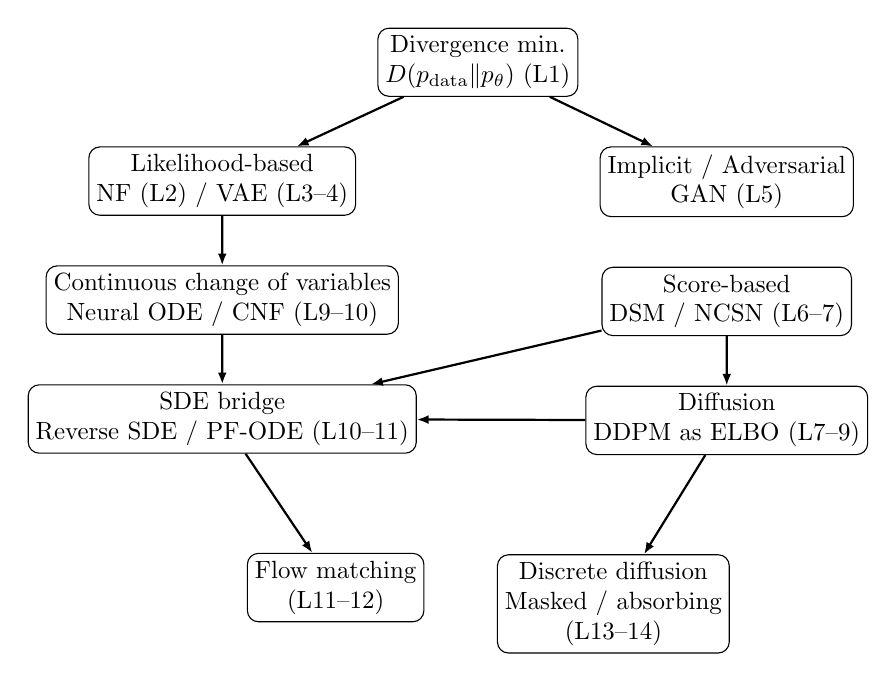
\begin{tikzpicture}[
		scale=0.9,
		transform shape,
		box/.style={draw, rounded corners, align=center, inner sep=3pt},
		arr/.style={-{Latex[length=1.5mm]}, thick},
		node distance=7mm and 3mm
	]
	\node[box] (div) {Divergence min.\\ $D(p_{\text{data}}\|p_\theta)$ (L1)};
	\node[box, below left=of div] (lik) {Likelihood-based\\ NF (L2) / VAE (L3--4)};
	\node[box, below right=of div] (imp) {Implicit / Adversarial\\ GAN (L5)};

	\node[box, below=of lik] (flows) {Continuous change of variables\\ Neural ODE / CNF (L9--10)};
	\node[box, below=of imp] (score) {Score-based\\ DSM / NCSN (L6--7)};

	\node[box, below=of flows] (sde) {SDE bridge\\ Reverse SDE / PF-ODE (L10--11)};
	\node[box, below=of score] (ddpm) {Diffusion\\ DDPM as ELBO (L7--9)};

	\node[box, below=14mm of sde, xshift=16mm] (fm) {Flow matching\\ (L11--12)};
	\node[box, below=14mm of ddpm, xshift=-16mm] (disc) {Discrete diffusion\\ Masked / absorbing\\ (L13--14)};

	\draw[arr] (div) -- (lik);
	\draw[arr] (div) -- (imp);
	\draw[arr] (lik) -- (flows);
	\draw[arr] (score) -- (ddpm);
	\draw[arr] (flows) -- (sde);
	\draw[arr] (ddpm) -- (sde);
	\draw[arr] (sde) -- (fm);
	\draw[arr] (ddpm) -- (disc);
	\draw[arr] (score) -- (sde);
	\end{tikzpicture}
\end{frame}
%=======
\begin{frame}{Comparison Cheat-Sheet: Part 1}
	\renewcommand{\arraystretch}{1.5}
	\center
	\begin{tabular}{lcccc}
		\hline
		\textbf{Family} & \textbf{Likelihood} & \textbf{Training} \\
		\hline
		AR & \checkmark & stable CE \\
		NF & \checkmark & tricky architecture \\
		VAE & lower bound & stable ELBO \\
		GAN & $\times$ & unstable/minimax \\
		Diffusion & bound / est. & stable \\
		FM / ODE & est. / bound & stable \\
		Discr. diff. & bound / CE-like & stable \\
		\hline
	\end{tabular}
\end{frame}
%=======
\begin{frame}{Comparison Cheat-Sheet: Part 2}
	\renewcommand{\arraystretch}{1.5}
	\center
	\begin{tabular}{lcccc}
	\hline
	\textbf{Family} & \textbf{Sampling} & \textbf{Best for} \\
	\hline
	AR & slow (sequential) & text / discrete \\
	NF & fast (1 step) & exact density, OOD \\
	VAE & fast (1 step) & latent modelling \\
	GAN & fast (1 step) & sharp images \\
	Diffusion & slow (many steps) & high fidelity + diversity \\
	FM / ODE & medium--fast & fewer steps + theory \\
	Discr. diff. & iterative & sequences + bidirectional gen \\
	\hline
	\end{tabular}
\end{frame}
%=======
\begin{frame}{Generative Learning Trilemma}
	\myfootnotewithlink{https://arxiv.org/abs/2112.07804}{Xiao Z., Kreis K., Vahdat A. Tackling the generative learning trilemma with denoising diffusion GANs, 2021}
	\begin{figure}
		\includegraphics[width=0.7\linewidth]{figs/trilemma}
	\end{figure}
\end{frame}
%=======
\begin{frame}{Generative Learning Trilemma}
	\begin{block}{Rule of Thumb}
	\small
		\begin{itemize}
			\item \textbf{Likelihood $\;\&\;$ Coverage} $\Rightarrow$ 
			\textbf{AR / NF}  
			\hfill exact density, no mode dropping, \textit{slow sampling}

			\item \textbf{Likelihood $\;\&\;$ Fast Sampling} $\Rightarrow$ 
			\textbf{VAE}  
			\hfill tractable bound, fast, \textit{blurry samples}

			\item \textbf{Sample Quality $\;\&\;$ Fast Sampling} $\Rightarrow$ 
			\textbf{GAN}  
			\hfill sharp samples, \textit{no likelihood, mode collapse}

			\item \textbf{Quality $\;\&\;$ Coverage} $\Rightarrow$ 
			\textbf{Diffusion}  
			\hfill stable training, high fidelity, \textit{slow sampling}

			\item \textbf{Quality $\;\&\;$ Faster Sampling} $\Rightarrow$ 
			\textbf{FM / ODE}  
			\hfill fewer steps, continuous flows, \textit{approx.\ likelihood}

			\item \textbf{Discrete Structure $\;\&\;$ Coverage} $\Rightarrow$ 
			\textbf{Discrete Diffusion}  
			\hfill stable CE training, parallel denoising, \textit{iterative decoding}
		\end{itemize}
	\end{block}
\end{frame}
%=======
\begin{frame}{Summary}
	\begin{itemize}
		\item For sequences, the forward process of discrete diffusionfactorize over positions, but
		reverse process (the model $\pt$) conditions on the whole context.
		\vfill
		\item In the absorbing case, tokens are either unchanged or masked; so only masked tokens contribute to the ELBO loss.
		\vfill
		\item The discrete ELBO reduces to a MLM objective.
		\vfill
		\item Reparameterizing time by the mask rate $\lambda\in[0,1]$ yields a continuous mixture of MLM losses.
		\vfill
		\item MDLM sampling performs iterative parallel refinement from fully masked to fully unmasked sequences.
		\vfill
		\item No generative model is strictly better than all others: different methods occupy different corners of the generative learning trilemma and come with unavoidable disadvantages.
	\end{itemize}
\end{frame}
%=======
\end{document}